\documentclass[letterpaper,12pt,oneside,onecolumn]{article}
\usepackage[margin=1in, bottom=1in, top=1in]{geometry} %1 inch margins
\usepackage{amsmath, amssymb, amstext}
\usepackage{fancyhdr}
\usepackage{mathtools}
\usepackage{algorithm}
\usepackage{algpseudocode}
\usepackage{theorem}
\usepackage{tikz}
\usepackage{tkz-berge}

%Macros
\newcommand{\A}{\mathbb{A}} \newcommand{\C}{\mathbb{C}}
\newcommand{\D}{\mathbb{D}} \newcommand{\F}{\mathbb{F}}
\newcommand{\N}{\mathbb{N}} \newcommand{\R}{\mathbb{R}}
\newcommand{\T}{\mathbb{T}} \newcommand{\Z}{\mathbb{Z}}
\newcommand{\Q}{\mathbb{Q}}
 
 
\newcommand{\cA}{\mathcal{A}} \newcommand{\cB}{\mathcal{B}}
\newcommand{\cC}{\mathcal{C}} \newcommand{\cD}{\mathcal{D}}
\newcommand{\cE}{\mathcal{E}} \newcommand{\cF}{\mathcal{F}}
\newcommand{\cG}{\mathcal{G}} \newcommand{\cH}{\mathcal{H}}
\newcommand{\cI}{\mathcal{I}} \newcommand{\cJ}{\mathcal{J}}
\newcommand{\cK}{\mathcal{K}} \newcommand{\cL}{\mathcal{L}}
\newcommand{\cM}{\mathcal{M}} \newcommand{\cN}{\mathcal{N}}
\newcommand{\cO}{\mathcal{O}} \newcommand{\cP}{\mathcal{P}}
\newcommand{\cQ}{\mathcal{Q}} \newcommand{\cR}{\mathcal{R}}
\newcommand{\cS}{\mathcal{S}} \newcommand{\cT}{\mathcal{T}}
\newcommand{\cU}{\mathcal{U}} \newcommand{\cV}{\mathcal{V}}
\newcommand{\cW}{\mathcal{W}} \newcommand{\cX}{\mathcal{X}}
\newcommand{\cY}{\mathcal{Y}} \newcommand{\cZ}{\mathcal{Z}}

\newcommand\numberthis{\addtocounter{equation}{1}\tag{\theequation}}


\newenvironment{proof}{{\bf Proof:  }}{\hfill\rule{2mm}{2mm}}
\newenvironment{proofof}[1]{{\bf Proof of #1:  }}{\hfill\rule{2mm}{2mm}}
\newenvironment{proofofnobox}[1]{{\bf#1:  }}{}\newenvironment{example}{{\bf Example:  }}{\hfill\rule{2mm}{2mm}}

%\renewcommand{\thesection}{\lecnum.\arabic{section}}
%\renewcommand{\theequation}{\thesection.\arabic{equation}}
%\renewcommand{\thefigure}{\thesection.\arabic{figure}}

\newtheorem{fact}{Fact}[section]
\newtheorem{lemma}[fact]{Lemma}
\newtheorem{theorem}[fact]{Theorem}
\newtheorem{definition}[fact]{Definition}
\newtheorem{corollary}[fact]{Corollary}
\newtheorem{proposition}[fact]{Proposition}
\newtheorem{claim}[fact]{Claim}
\newtheorem{exercise}[fact]{Exercise}
\newtheorem{note}[fact]{Note}
\newtheorem{conjecture}[fact]{Conjecture}

\newcommand{\size}[1]{\ensuremath{\left|#1\right|}}
\newcommand{\ceil}[1]{\ensuremath{\left\lceil#1\right\rceil}}
\newcommand{\floor}[1]{\ensuremath{\left\lfloor#1\right\rfloor}}

%END MACROS
%Page style
\pagestyle{fancy}

\listfiles

\raggedbottom

\lhead{2017-02-17}
\rhead{W. Justin Toth CS798-Convexity and Optimization Assignment 1} %CHANGE n to ASSIGNMENT NUMBER ijk TO COURSE CODE
\renewcommand{\headrulewidth}{1pt} %heading underlined
%\renewcommand{\baselinestretch}{1.2} % 1.2 line spacing for legibility (optional)

\begin{document}
%Q1%
\section{}
\paragraph{}
Let $q > p > 0$ and let $x_1, \dots, x_n \in \R_{>0}$. Let $f : \R_{>0} \rightarrow \R_{>0}$ be the function given by $f(x) = x^\frac{q}{p}$. We claim that $f$ is convex. To see this we will use the second order condition ($f'' \geq 0$). We have by calculus that
$$f' (x)= \frac{q}{p} x^{\frac{q}{p}-1}$$
and thus 
$$f''(x) = \frac{q}{p}(\frac{q}{p} -1) x^{\frac{q}{p} - 2}.$$
Now since $q > p$, we have $\frac{q}{p} > 1$. So then $\frac{q}{p} - 1$ is non-negative, and further $x^{\frac{q}{p} - 2} > 0$ since $x >0$. Hence $f''(x) \geq 0$ on the domain of $f$. Therefore by the second order condition, $f$ is convex.
\paragraph{}
Now observe by convexity that
$$f(\frac{1}{n}\sum_{i=1}^n x_i^p) \leq \frac{1}{n} \sum_{i=1}^n f(x_i^p) = \frac{1}{n} \sum_{i=1}^n x_i^q.$$
On the other hand, by applying $f$ directly we see that
$$f(\frac{1}{n}\sum_{i=1}^n x_i^p) = \frac{1}{n}^\frac{q}{p}(\sum_{i=1}^n x_i^p)^\frac{q}{p}.$$
Combining the previous two expressions yields the inequality
$$\frac{1}{n}^\frac{q}{p}(\sum_{i=1}^n x_i^p)^\frac{q}{p} \leq \frac{1}{n} \sum_{i=1}^n x_i^q.$$
By raising both sides to the exponent $\frac{1}{q}$ (which preserves order) we obtain that
$$(\frac{1}{n}\sum_{i=1}^n x_i^p)^\frac{1}{p} \leq (\frac{1}{n} \sum_{i=1}^n x_i^q)^\frac{1}{q}$$
as desired. $\blacksquare$
%Q2
\section{}
%Pa
\subsection{a}
\paragraph{}
Consider the function
$$f(x) = (\sum_{i=1}^n x_i^p)^\frac{1}{p}$$
with $\text{dom} f = \R^n_{>0}$. We will compute the Hessian matrix. First observe that
$$\frac{\partial f}{\partial x_i} f = x_i^{p-1}(\sum_{k=1}^n x_k^p)^\frac{1-p}{p}$$
for $i = 1, \dots, n$. Now for $j = 1, \dots, n$
\begin{align*}
\frac{\partial f}{\partial x_j}\frac{\partial f}{\partial x_i} f &= \frac{\partial f}{\partial x_j}   x_i^{p-1}(\sum_{i=1}^n x_i^p)^\frac{1-p}{p} \\
&=(p-1)(\sum_{k=1}^n x_k^p)^\frac{1-2p}{p}\begin{cases}
-x_i^{p-1}x_j^{p-1}, &i\neq j \\
x_i^{p-2}\sum_{k=1}^n x_k^p  -x_i^{p-1}x_j^{p-1}, &i=j.
\end{cases}
\end{align*}
We claim that the Hessian is positive semidefinite. We prove this directly from the definition, let $y \in \R^n$:
\begin{align*}
y^T\nabla^2f(x)y &= \sum_{i=1}^n \sum_{j=1}^n \nabla^2f(x)_{ij} y_i y_j \\
&= (p-1) (\sum_{k=1}^nx^p)^\frac{1-2p}{p}[\sum_{i=1}^nx_i^{p-2}(\sum_{k=1}^nx_k^p)y_i^2 - \sum_{i=1}^n\sum_{j=1}^n x_i^{p-1}x_j^{p-1}y_i y_j ] \\
&= (p-1) (\sum_{k=1}^nx^p)^\frac{1-2p}{p}[(\sum_{i=1}^nx_i^{p})(\sum_{i=1}^nx_i^{p-2}y_i^2) - (\sum_{i=1}^n x_i^{p-1}y_i)(\sum_{i=1}^n x_i^{p-1} y_i) ] \\
&= (p-1) (\sum_{k=1}^nx^p)^\frac{1-2p}{p}[(\sum_{i=1}^nx_i^{p})(\sum_{i=1}^nx_i^{p-2}py_i^2) - (\sum_{i=1}^n x_i^\frac{p}{2}x_i^\frac{p-2}{2}y_i)(\sum_{i=1}^n x_i^\frac{p}{2}x_i^\frac{p-2}{2}y_i)]\\
&= (p-1) (\sum_{k=1}^nx^p)^\frac{1-2p}{p}[(\sum_{i=1}^nx_i^{p})(||x^\frac{p}{2}||^2||x^\frac{p-2}{2}y||^2 - \langle x^\frac{p}{2}, x^\frac{p-2}{2}y\rangle^2]
\geq 0.
\end{align*}
The inequality follows since $p-1 \geq 1$ (as $p \geq 1$), $(\sum_{k=1}^nx^p)^\frac{1-2p}{p} \geq 0$ (as $x \in \R^n_{>0}$), and 
$$||x^\frac{p}{2}||^2||x^\frac{p-2}{2}y||^2 \geq \langle x^\frac{p}{2}, x^\frac{p-2}{2}y\rangle^2$$
by Cauchy-Schwarz. Hence $\nabla^2f(x)$ is positive semidefinite and thus by the Second Order Condition, (since $\R^n_{>0}$ is open) $f$ is convex.
\paragraph{}
Now when $p < 1$, by a similar calculation we observe
\begin{align*}
\frac{\partial -f}{\partial x_j}\frac{\partial f}{\partial x_i} f &=(1-p)(\sum_{k=1}^n x_k^p)^\frac{1-2p}{p}\begin{cases}
-x_i^{p-1}x_j^{p-1}, &i\neq j \\
x_i^{p-2}\sum_{k=1}^n x_k^p  -x_i^{p-1}x_j^{p-1}, &i=j.
\end{cases}
\end{align*}
So again calculating the quadratic form $y^T\nabla^2-f(x)y$ we have
\begin{align*}
y^T\nabla^2-f(x)y &=(1-p) (\sum_{k=1}^nx^p)^\frac{1-2p}{p}[(\sum_{i=1}^nx_i^{p})(||x^\frac{p}{2}||^2||x^\frac{p-2}{2}y||^2 - \langle x^\frac{p}{2}, x^\frac{p-2}{2}y\rangle^2]\\
&\geq 0.
\end{align*}
Since $p < 1$, $1-p >0$, and so the inequality follows as before. Therefore, by the Second Order Condition $-f$ is convex, and hence $f$ is concave. $\blacksquare$
\paragraph{}
Next we show that
$$||x||_p = (\sum_{i=1}^n |x_i|^p)^\frac{1}{p}$$
is a norm for $p\geq 1$. It is easy to see that $||x||_p$ is non-negative since it is a sum of absolute values. Similarly if any $x_i > 0$ then $||x||_p > 0$, so $||x||_p = 0$ if and only if $x = 0$. Now consider some scalar $\alpha$. We have
$$||\alpha x||_p = (\sum_{i=1}^n |\alpha x_i|^p)^\frac{1}{p} = (\sum_{i=1}^n |\alpha|^p|\cdot |x_i|^p)^\frac{1}{p} = |\alpha|(\sum_{i=1}^n |x_i|^p)^\frac{1}{p} = |\alpha|\cdot ||x||_p.$$
\paragraph{}
Lastly it remains to verify the triangle inequality. Let $x, y \in \R^n$. If either $x$ or $y$ is $0$, say without loss of generality $y=0$, then 
$$||x + y||_p = ||x||_p + 0 = ||x||_p + ||y||_p$$
immediately. So we may assume $x$ and $y$ are non-zero. Thus it suffices to prove
$$f(x+y) \leq f(x) + f(y).$$
To show this we exploit convexity of $f$ as follows
$$f(x+y) = f(\frac{1}{2}(2x+2y)) \leq \frac{1}{2}(f(2x) + f(2y)) = \frac{1}{2} ((2^p\sum_{i=1}^n x^p)^\frac{1}{p} +(2^p\sum_{i=1}^n y^p)^\frac{1}{p}) = f(x) + f(y).$$
Therefore $||x + y||_p \leq ||x||_p + ||y||_p$, and hence $||x||_p$ is a norm. $\blacksquare$
\paragraph{}
Finally we give a counter-example showing $||x||_p$ is not a norm when $0 < p < 1$. Consider $p =\frac{1}{2}$ and $e_1, e_2 \in \R^2$ the standard basis vectors of $\R^2$. We prove $||x||_p$ violates the triangle inequality. Observe
$$||e_1 + e_2 ||_p = (1 + 1)^2 = 4$$
while 
$$||e_1|| = (1+0)^2 = 1 = ||e_2||$$
hence 
$$||e_1 + e_2||  = 4 < 2 = ||e_1|| + ||e_2||.$$
Thus the triangle inequality is violated, and so $||x||_p$ is not a norm.
%Pb
\subsection{b}
\paragraph{}
Let $n \in \N$ and consider the function $f: S^n_{++} \rightarrow \R$ given by
$$f(x) = (\det X)^\frac{1}{n}.$$
We will demonstrate that $f$ is concave. It suffices to show that the function 
$$g(t) = (\det (Z + t V))^\frac{1}{n} $$
is concave for arbitrary $Z \in S^n_{++}$ and $V \in S^n$. Note that $g$ is the restriction of $f$ to some arbitrary line. The domain of $g$ is $\{t \in \R: Z + tV \in S^n_{++}\}$.
\paragraph{}
Since $Z \in S^n_{++}$ we can decompose $Z$ as $Z=Z^\frac{1}{2}Z^\frac{1}{2}$ with $Z^\frac{1}{2}$ non-singular. Let $\lambda_1, \dots, \lambda_n$ denote the eigenvalues of $Z^\frac{-1}{2}VZ^\frac{-1}{2}$. Then we observe that
$$g(t) = (\det(Z+tV))^\frac{1}{n} = (\det(Z^\frac{1}{2}(I + tZ^\frac{-1}{2}VZ^\frac{-1}{2})Z^\frac{1}{2}))^\frac{1}{n}.$$
Using that $\det(\cdot)$ distributes over matrix products and that $\det(A)$ is equal to the product of the eigenvalues of $A$ we have
$$g(t) = \det(Z^\frac{1}{2})^\frac{2}{n}\det(1 + tZ^\frac{-1}{2}VZ^\frac{-1}{2}) = \det(Z^\frac{1}{2})^\frac{2}{n}(\Pi_{i=1}^n 1+t\lambda_i)^\frac{1}{n}.$$
Now we will show that $g$ is a composition of affine and concave functions, and hence that $g$ is concave. Let $h : \R \rightarrow \R^n$ be the affine function given by
$$h(t)_i = 1+t\lambda_i$$
for $i = 1\dots n$. Let $ y : \R^n \rightarrow \R$ be the geometric mean function
$$y(x) = (\Pi_{i=1}^n x_i)^\frac{1}{n}.$$
We know from the notes that $y$ is concave. Finally, let $z: \R\rightarrow \R$ be the affine (linear actually) function given by
$$z(x) = \det(Z^\frac{1}{2})^\frac{2}{n}$$
Then we see that
$$g(t) = z\circ y\circ h(t).$$
Thus $g$ is a composition of affine functions with a concave function and hence $g$ is concave.$\blacksquare$
%Q3
\section{}
\paragraph{}
Let $f : \R^n \rightarrow \R$ be a convex function and let $g : \R^n \rightarrow \R$ be a concave function with $\text{dom } f = \text{dom } g = \R^n$. Suppose that $g(x) < f(x)$ for all $x$. Let $e(f) = \{(x,t) \in \R^n \times \R: t \geq f(x) \}$ be the epigraph of $f$. We know from our notes that $e(f)$ is convex. Let $b(f) = \{(x,t) \in \R^n \times \R: t \leq g(x)\}$ denote the ``below" graph (sorry I don't know the technical name of this object) of $g$. We claim that $b(g)$ is convex.
\paragraph{}
Let $(x_1, t_1), (x_2, t_2) \in b(g)$. Then we have
\begin{align*}
-g(\frac{1}{2}(x_1 + x_2)) &\leq \frac{1}{2}(-g(x_1) - g(x_2)) &\text{ since $-g$ is convex} \\
&=\frac{-1}{2}(g(x_1) + g(x_2)).
\end{align*}
Multiplying by $(-1)$, then using that $x_1, t_1), (x_2, t_2) \in b(g)$ we obtain
$$g(\frac{1}{2}(x_1 + x_2)) \geq \frac{1}{2}(g(x_1) + g(x_2)) \geq \frac{1}{2}(t_1 + t_2).$$
Thus $\frac{1}{2}[(x_1,t_1) + (x_2,t_2)] \in b(g)$, that is to say $b(g)$ is convex.
\paragraph{}
Now we claim that $e(f) \cap b(g) = \emptyset$. Suppose for a contradiction that there exists $(x,t) \in e(f) \cap b(g)$. Thus we have
$$t \geq f(x) \quad \text{and}\quad t \leq g(x).$$
But then $f(x) \leq g(x)$, contradicting that $f(x) > g(x)$ for all $x$. Thus $e(f)$ and $b(g)$ are disjoint.
\paragraph{}
Using the Separating Hyperplane Theorem as written in section $2.5.1$ of Boyd and Vandenberghe, on $e(f)$ and $b(g)$ we observe that there exists $(y,a) \in \R^n \times \R$ and $b \in \R$, a hyperplane, which separates $e(f)$ and $b(g)$:
\begin{align}
y^Tx + at &\geq b &\forall (x,t) \in e(f) \label{eq:3.1}\\
y^Tx + at &\leq b &\forall (x,t) \in b(g) \label{eq:3.2}.
\end{align}
Now we verify that $a\geq 0$. Let $x \in \R^n$. Then applying $\ref{eq:3.1}$ to $(x,f(x))$ and $\ref{eq:3.2}$ to $(x,g(x))$ and applying transitivity through $b$ we have
$$y^Tx + af(x) \geq y^Tx + ag(x)$$
Thus
$$a(f(x) - g(x)) \geq 0.$$
Since $f(x) > g(x)$ this implies
$$a \geq 0.$$
Now observe that
$$y^Tx + af(x) \geq b$$
implies
$$ f(x) \geq \frac{b}{a} - \frac{y^Tx}{a}$$
and
$$ y^Tx + ag(x) \leq b$$
implies 
$$g(x) \leq \frac{b}{a} - \frac{y^Tx}{a}.$$
Let $h(x): \R^n \rightarrow \R$ be the affine function given by
$$h(x) =\frac{-1}{a}(y^Tx - b)$$
Then we have immediately
$$g(x) \leq h(x) \leq f(x)$$
for all $x \in \R^n$ as desired. $\blacksquare$

%Q4
\section{}
\paragraph{}
Let $P = \{ x| Ax \leq b\}$ be a polytope, where $A \in \R^{m\times n}$, $b \in \R^m_{>0}$. Let $a_i$ denote the $i$-th row of $A$. Let $[m] = \{1,\dots, m\}$. Let $C = \text{conv} \{\frac{a_i}{b_i} : i\in [m]\}$ be the convex hull of $\frac{a_i}{b_i}$'s. We want to show that $P^* = C$, where $P^*$ denotes the polar set of $P$.
\paragraph{}
We will use the theorem from class that $P^{**} = P$ when $0 \in P$. With this theorem it is equivalent to show that $P = C^*$. First we will rewrite $P$ as $P = \{x| a_i^Tx \leq b_i \forall i\in[m]\}$. Observe that 
$$C^* := \{ x: x^Ty \leq 1\forall y \in C\}.$$
Observe that $\forall y \in C$ there exists $\lambda_i$ for $i\in [m]$ such that $y = \sum_{i\in[m]} \lambda_i \frac{a_i^T}{b_i}$, $\sum_{i\in [m]}\lambda_i = 1$, and $\lambda \geq 0$. This is the definition of convex hull. Hence substituting into our definition of $C^*$ we see
$$C^* = \{x : x^T(\sum_{i} \lambda_i \frac{a_i^T}{b_i}) \leq 1,\ \forall \lambda \geq 0, \sum_i \lambda_i = 1\}.$$
Rewriting slightly this is equivalent to
$$C^* = \{x : \sum_{i}\lambda_i \frac{a_i}{b_i}x \leq 1,\ \forall \lambda \geq 0, \sum_i\lambda_i = 1\}.$$
It is not hard to see that such $C^* = P$. We will write it out formally below for the sake of completeness.
\paragraph{}
Let $x\in C^*$. Then if we for each $i \in [m]$ define the vector $\lambda^i$ as
$$\lambda^i_j = \begin{cases}
1, &i=j \\
0, &i\neq j.
\end{cases}$$
Then $\lambda^i \geq 0$ and $\sum_j \lambda^i_j = \lambda^i_i = 1$. Since $x \in C$ we have
$$\sum_{j}\lambda^i_j \frac{a_j}{b_j} x \leq 1$$
and hence
$$\frac{a_i}{b_i} x \leq 1.$$
Thus for all $i \in [m]$, $a_i x\leq b_i$ ($b_i > 0$ implies inequality does not change order) and therefore $x \in P$. Now if we let $x\in P$, and let $\lambda \geq 0$ such that $\sum_i \lambda_i = 1$ then we need to show that $\sum_i \lambda_i \frac{a_i}{b_i} x \leq 1$. Since $x \in P$, $a_i x \leq b_i$ for all $i \in [m]$. Dividing by $b_i$ and multiplying by $\lambda_i \geq 0$ we obtain
$$\lambda_i\frac{a_i}{b_i} x \leq \lambda_i \quad \forall i \in [m].$$
Summing these inequalities over $i\in[m]$ obtains the desired bound:
$$\sum_i \lambda_i \frac{a_i}{b_i}x \leq \sum_i \lambda_i = 1.$$
Thus $P= C^*$ and by our theorem, $P^* = C^{**} = C$. For this theorem to apply it remains to verify that $0 \in C$.
\paragraph{}
Suppose for a contradiction that $0 \not\in C$. Since $C$ is a convex hull of a finite set it is closed and bounded. Hence, by the separating hyperplane theorem there exists a (non-zero) hyperplane $h \in \R^n$ such that 
$$h^T0 > h^Tx \quad\forall x \in C.$$
We claim that $h$ is a direction in $P$. To see this let $\alpha \in \R$ be a scalar. Let $x \in P$.  We will show that $x + \alpha h$ is feasible, implying that $h$ is a direction in $P$. Let $ i \in [m]$ and consider constraint $a_i$ with $b_i$. Then
$$\frac{a_i}{b_i} (x + \alpha h) = \frac{a_i}{b_i}x + \alpha \frac{a_i}{b_i}h < \frac{a_i}{b_i}x \leq 1.$$
The first inequality follows since $\frac{a_i}{b_i} \in C$ (and thus $\frac{a_i}{b_i} h < h^T0 = 0)$ and the second inequality follows since $x \in P$. Thus multiplying through by $b_i$, which will not reverse the order of inequalities since $b_i > 0$, we obtain
$$\frac{a_i}(x + \alpha h) < b_i.$$
Since this holds for all $i \in [m]$ this implies that $x + \alpha h \in P$. Hence $h$ is a direction, contradicting that $P$ is bounded. Therefore $0\in C$ as desired. $\blacksquare$

%Q5
\section{}
Let $Q \in S^n_{++}$. We consider the quadratic norm $||x||_Q := (x^TQx)^\frac{1}{2}.$
%pa
\subsection{a}
\paragraph{}
We show that $||x||_Q$ is a norm. First since $Q\in S^n_{++}$ there exists non-singular, symmetric $V$ such that $Q = V^TV$. Observe that
$$||x||_Q = (x^TQx)^\frac{1}{2} = (x^TV^TVx)^\frac{1}{2} =  ((Vx)^T(Vx))^\frac{1}{2} = ||Vx||_2.$$
We will show that $||x||_Q$ is non-negative and equal to $0$ only when $x = 0$, that $||t x||_Q = |t|\cdot ||x||_Q$, and that triangle inequality holds.
\paragraph{Non-negativity}
Since $||\cdot||_2$ is a norm, $||x||_Q = ||Vx||_2 \geq 0$ and further $||Vx||_2 = ||x||_Q = 0$ only if $Vx = 0$, but then $x = V^{-1}0 = 0$.
\paragraph{Scaling}
Observe that $$||tx||_Q = ||V(tx)||_2 = |t|\cdot ||Vx||_2 = |t|\cdot ||x||_Q.$$
\paragraph{Triangle Inequality}
Let $x,y \in \R^n$. Then
$$||x+y||_Q = ||V(x+y)||_2 = ||Vx + Vy||_2 \leq ||Vx||_2 + ||Vy||_2 = ||x||_Q + ||y||_Q.$$
Therefore $||\cdot||_Q$ is a norm. $\blacksquare$
%pb
\subsection{b}
\paragraph{}
Let $x \in \R^n$. Then observe that
\begin{align*}
||x||_{Q^*} = \sup \{ x^Ty : ||y||_Q \leq 1\} \\
&= \sup \{x^Ty : ||Vy||_2 \leq 1\} \\
&= \sup \{x^TV^{-1}Vy : ||Vy||_2 \leq 1\} \\
&= \sup\{x^TV^{-1}z : ||z||_2 \leq 1\} &\text{assigning $z=Vy$}. 
\end{align*}
The supremum is realized when $z = (x^TV^{-1})^T = V^{-1}x$. Therefore
$$||x||_{Q^*} = x^TV^{-1}V^{-1}x = x^TQ^{-1}x = ||x||_{Q^{-1}}.$$
Thus our nice formula is $||x||_{Q^*} = ||x||_{Q^{-1}}$.$\blacksquare$
%pc
\subsection{c}
\paragraph{}
Let $\cE = \{x : x^TQx \leq 1\}.$  Rewriting we have $\cE = \{x : ||x||_Q \leq 1\} = \cB$ where $\cB$ denote the norm ball of $||\cdot||_Q$. Then we have
$$\cE^* = \{y : y^Tx \leq 1, \forall x \in \cE\} = \{y : y^Tx \leq 1, \forall x \in \cB\}  = \cB^* = \cB_*,$$
where $\cB_*$ is the norm ball of $||\cdot||_{Q^*}$, and the last equality follows from the notes. Rewriting using part $(b)$ we see that $\cB_* = \{x: x^TQ^{-1}x \leq 1\}$. That is $\cE^*$ is ellipsoid given by $Q^{-1}$.
\paragraph{}
So suppose $\cE$ is a $2D$-ellipsoid with semi-axes $v_1$ and $v_2$ with corresponding side lengths $a_1$ and $a_2$. Then the spectral decomposition of $Q$ is
$$Q = \begin{bmatrix} v_1 & v_2 \end{bmatrix} \begin{bmatrix} a_1^{-1} & 0 \\ 0 & a_2^{-1} \end{bmatrix} \begin{bmatrix} v_1^T \\v_2^T\end{bmatrix}.$$
And further
$$Q^{-1} =  \begin{bmatrix} v_1 & v_2 \end{bmatrix} \begin{bmatrix} a_1 & 0 \\ 0 & a_2 \end{bmatrix} \begin{bmatrix} v_1^T \\v_2^T\end{bmatrix}$$
using that $ \begin{bmatrix} v_1 & v_2 \end{bmatrix}^T =  \begin{bmatrix} v_1 & v_2 \end{bmatrix}^{-1}$. Hence the polar ellipsoid $\cE^*$ has the same semi-axes as $\cE$, but with reciprocal side lengths.
\begin{figure}[H]
\centering
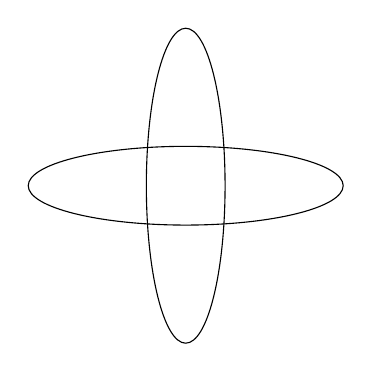
\begin{tikzpicture}
\draw (0,0) ellipse (0.5cm and 2cm);
\draw (0,0) ellipse (2cm and 0.5cm);
\end{tikzpicture}
\caption{Ellipsoid and its polar where $v_1 = e_1$ and $v_2 = e_2$ (standard basis vectors), and $a_1 = 2$ while $a_2 = \frac{1}{2}$. The polar scales $v_1$ by $\frac{1}{a_1} = \frac{1}{2}$ and scales $v_2$ by $\frac{1}{a_2} = 2$.}
\end{figure}

%Q6
\section{}
%Pa
\subsection{a}
\paragraph{}
Let $\cE_1:= \{P_1 u + q_1 : ||u||_2 \leq 1\}$ and $\cE_2:= \{P_2 u + q_2 : ||u||_2 \leq 1\}$ be given ellipsoids. We want to find a separating hyperplane $(a,b)$ for these ellipsoids, that is:
\begin{align*}
a^Tx + b &\geq 0 &\forall x \in \cE_1 \\
a^Tx+b &\leq 0 &\forall x \in \cE_2.
\end{align*}
This can be formulated as an optimization feasibility problem as
\begin{align*}
\min\ 0\\
\text{s.t.}\ a^Tx + b &\geq 0 &\forall x \in \cE_1\\
a^Tx + b &\leq 0 &\forall x \in \cE_2.
\end{align*}
This problem is equivalent to
\begin{align*}
\min\ 0\\
\text{s.t.}\ a^T(-x)&\leq b &\forall x \in \cE_1\\
a^Tx &\leq -b &\forall x \in \cE_2.
\end{align*}
Which is equivalent to
\begin{align*}
\min\ 0\\
\text{s.t.}\  
\sup\{ a^T(-x) : x \in \cE_1\}&\leq b\\
\sup\{a^Tx : x\in \cE_2\} &\leq -b.
\end{align*}
Equivalently
\begin{align*}
\min\ 0\\
\text{s.t.}\  
\sup\{ a^T(-P_1 u - q_1) : ||u||_1 \leq 1\}&\leq b\\
\sup\{a^T(P_2 u + q_2) : ||u||_2 \leq 1\} &\leq -b.
\end{align*}
Which is equivalent to
\begin{align*}
\min\ 0\\
\text{s.t.}\  
a^T(-q_1) + ||P_1a||_2 &\leq b\\
a^Tq_2 + ||P_2a||_2 &\leq -b.
\end{align*}
Setting $A_1 = P_1$, $b_1 = 0$, $c_1=q_1$, $d_1 = b$, and $A_2 = P_2$, $b_2 = 0$, $c_2 = -q_2$, and $d_2 = -b$ we obtain the exact form of a Second Order Conic Program as described in the general formulation of such problems. $\blacksquare$
\subsection{b}
\paragraph{}
We will write the Second-Order Cone Program (SOCP):
\begin{align*}
\min &f^Tx \\
\text{s.t.} ||A_ix + b_i||_2 &\leq c^T_i x + d_i, &1\leq i \leq m \\
Fx &= g,
\end{align*}
as a Semidefinite Program (SDP) in inequality form (see section $4.6.2$ of Boyd and Vandenberghe) :
\begin{align*}
\min\ &f^Tx \\
\text{s.t.}\ G + \sum_{i=1}^n x_i F_i &\preccurlyeq 0 \\
Fx &=g.
\end{align*}
Observe that it is enough to show that a constraint of the form $||Ax + b|| \leq c^Tx + d$ can be written as $G + \sum_{i=1}^n x_i F_i \preccurlyeq 0$ as then we could write each constraint $||A_ix + b_i||_2 \leq c^T_i x + d_i$ for $i\in [m]$ as $G^i + \sum_{j=1} x_j F^i_j$, and stack them as blocks as
$$G = \begin{bmatrix} G^1 & & \\ & \ddots & \\ & & G^m \end{bmatrix} \quad F_i = \begin{bmatrix} F^1_i & & \\ & \ddots & \\ & & F^m_i \end{bmatrix}$$
to obtain an equivalent single semidefinite constraint in place of $m$ semidefinite constraints.
\paragraph{Lemma 6b}
We will need the following lemma using Schur's complement: For any $x\in \R^n$ and $c\in \R$ we have $||x||_2 \leq c$ if and only if
$$X = \begin{bmatrix} c &x^T \\ x & cI\end{bmatrix} \succcurlyeq 0.$$
\paragraph{Proof of Lemma 6b}
If $c = 0$ this is trivial, so we may assume that $c\neq 0$. In this case we invoke Schur's Complement Lemma and thus
$$X \succcurlyeq 0$$
if and only if $c \geq 0$ and $tI - \frac{1}{c}xx^T \succcurlyeq 0$. Which holds if and only if $c^2I - xx^T \succcurlyeq 0$. Now the eigenvalues of $c^2I - xx^T$ are non-negative if and only if $c^2 - ||x||^2_2 \geq 0$ (since $c^2$ is the least eigenvalue of $c^2I$ and $||x^2_2$ is the largest eigenvalue of $xx^T$), which holds if and only if $||x||_2 \leq c$ as desired. $\blacksquare$
\paragraph{}
Now applying Lemma $6b$ to our SOCP cone constraint we have $||Ax +b||_2 \leq c^Tx + d$ (suppose $x\in\R^n$ and $A \in \R^{r\times n}$) if and only if
$$\begin{bmatrix} c^Tx + d & (Ax+b)^T \\ Ax + b &(c^T+d)xI \end{bmatrix} \succcurlyeq 0.$$
Let $a^1, \dots, a^r$ be the rows of $A$. Separating out we obtain:
$$\begin{bmatrix} d & b^T \\ b & dI \end{bmatrix} + \sum_{i=1}^n x_i \begin{bmatrix} c_i & a^1_i & \dots & a^r_i \\ a^1_i \\ \vdots & &c_iI\\ a^r_i \end{bmatrix} \succcurlyeq 0.$$
Thus setting $$G = -\begin{bmatrix} d & b^T \\ b & dI \end{bmatrix}$$
and 
$$F_i = -\begin{bmatrix} c_i & a^1_i & \dots & a^r_i \\ a^1_i \\ \vdots & &c_iI\\ a^r_i \end{bmatrix}$$
we have
$$G + \sum_{i=1}^n F_i \preccurlyeq 0$$
if and only if
$$||Ax+b||_2 \leq c^Tx + d.$$
Therefore we have shown that any SOCP can be written as an SDP. $\blacksquare$

%Q7
\section{}
\paragraph{}
Consider the following optimization problem $(P)$:
\begin{align*}
\min\ &e^{-x} \\
\text{s.t.}\ \frac{x^2}{y} &\leq 0,
\end{align*}
with domain $\cD = \{(x,y) : y > 0 \}$. The Lagrangian function $g(\lambda)$ is
$$ g(\lambda) := \inf_{x,y} \{ e^{-x} + \lambda \frac{x^2}{y}\}.$$
We will study the behaviour of $g$ to understand the value of the dual problem.
\paragraph{}
The dual problem $(D)$ is:
\begin{align*}
\max\ &g(\lambda) \\
\lambda &\geq 0.
\end{align*}
We consider two cases: when $\lambda = 0$ and when $\lambda > 0$.
\paragraph{}
When $\lambda = 0$, 
$$g(\lambda) = \inf_x e^{-x} = 0.$$
Now when $\lambda > 0$ observe that $y = \lambda x^4 > 0$ for $x > 0$ and so
$$\lim_{x \rightarrow \infty, y=x^4} (e^{-x} + \lambda\frac{x^2}{y}) = \lim_{x\rightarrow \infty} (e^{-x} + \lambda\frac{x^2}{\lambda x^4}) = \lim_{x\rightarrow \infty}( e^{-x} + \frac{1}{x^2}) = 0.$$
Since $g(\lambda) \geq 0$ this implies $g(\lambda) = 0$. Therefore in either case $g(\lambda) = 0$. Thus $(D)$ is equal to:
\begin{align*}
\max\ &0 \\
\lambda &\geq 0.
\end{align*}
And thus if we let$d^*$ be the optimal value of $(D)$, then $d^*=0$.
\paragraph{}
Now we return our attention to $(P)$. Since $x^2 \geq 0$ for all $x$ and $y > 0$ we observe that
$$\frac{x^2}{y} \leq 0 \iff x = 0.$$
Thus all feasible $(x,y)$ for $(P)$ have objective value $e^{-0} = 1$. So if we let $p^*$ be the optimal value of $(P)$ then $p^* = 1$.
\paragraph{}
Therefore $p^* = 1 > 0 = d^*$, so strong duality does not hold for this problem. $\blacksquare$
\end{document}